\chapter{Sequence prediction with traces}
\label{chap:taking-inspiration}
Previous works have demonstrated the practicality of LSTM neural networks for Predictive Process Monitoring. However, only the use of Embedding layers was inspired by Natural Language Processing (NLP) until now~\cite{evermann2016}. We believe that more knowledge could be transferred because both domains revolve around sequential data. In this chapter, we outline how we take inspiration from sequence prediction in NLP, and thus contribute to Improvement Area 3 from \autoref{sec:intro:motivation}.

We establish the connection between traces and sequences by connecting their definitions in \autoref{sec:contrib:case-sequence-understanding}. This provides the underpinning for introducing two NLP-inspired approaches for predicting the next activity in a case. These approaches are presented in \autoref{sec:contrib:sp2-inspiration} and \autoref{sec:contrib:pfs-inspiration}.

\section{Understanding traces as sequences}\label{sec:contrib:case-sequence-understanding}
The definition for sequences presented in \autoref{sec:background:sequences} and the definition of traces in \autoref{sec:log-structure} will be connected in this section to make it clear how events can be understood as itemsets.

Each case $c$ contains its execution history in its trace attribute $\#_{trace}(c)$.
Both a trace $\#_{trace}(c)$ and a sequence $seq$ are defined to contain ordered data:

\begin{equation*}
\begin{split}
seq           &=  \langle s_1,s_2\cdots s_l \rangle\ |\ \forall\ 1 \leq j \leq l: s_j \subseteq \mathscr{I}\\
\#_{trace}(c) &= \langle e_1, e_2, e_3\cdots e_n \rangle
\end{split}
\end{equation*}

An itemset $s = (i_1, i_2 \cdots i_n)$ consists of items $i \in \mathscr{I}$.
An event $e$ is made up of attributes that are accessed via the $\#$ operator.
It can be said that both itemsets and events act as containers of information.
Therefore, we connect the definitions of the contained information in a first step.
The set of items $\mathscr{I}$ is then defined as the set of all attributes of all events in all cases in a given log $L$:

$$\mathscr{I} = \{\#_{a}(e)\ |\ c \in L\wedge e \in \#_{trace}(c) \wedge a \in attribute\_names(e)\}$$

Itemsets are defined $s \subseteq \mathscr{I}$.
This does not place any restrictions on the content of $s$,
and so an itemset could consist only out of timestamps.
To preven such cases, we introduce a schema on the itemsets in a second step.
It is introduced as a direct mapping from an event $e$ to an itemset $s$:

$$ s = (i_1, i_2 \cdots i_n)\ |\ i_k = \#_{attribute\_names_k(e)}(e), 1 \leq k \leq n $$

The definition places each item $i_k$ on a specific place in the itemset, depending on the index $k$ in the attribute list $attribute\_names(e)_k$.
The original condition $s \subseteq \mathscr{I}$ hold true.
This definition enables sequence prediction on traces, and also provides the tabular format required for machine learning.

In \autoref{sec:background:sequence-prediction}, a many-to-one prediction is defined to target the next itemset $\widehat{s_{k+1}}$ of $seq_{1,k}$.
In the use case at hand, that would entail the prediction of all data attributes in $s_{k+1}$.
Since we specifically target the name of the next activity, we adjust the definition of the prediction function to target a single item $\hat{i_j}$. The index $j$ corresponds to the column index of the target variable inside the itemset $s_{k+1}$.

$$ predict(seq_{1,k}) = \hat{i_j} $$

With the prediction target at hand, we move on to present the network architectures for executing the prediction.

\section{Adapting a competition submission}\label{sec:contrib:sp2-inspiration}
Shibata et al.'s bipartite network architecture has shown outstanding performance in the Sequence Prediction competition (SPiCe)~\cite{web:spice}.
Under the assumption that a case can exhibit properties similar to sentences, we adapt it for use in the business process domain.

\begin{figure}[!htb]
    \centering
    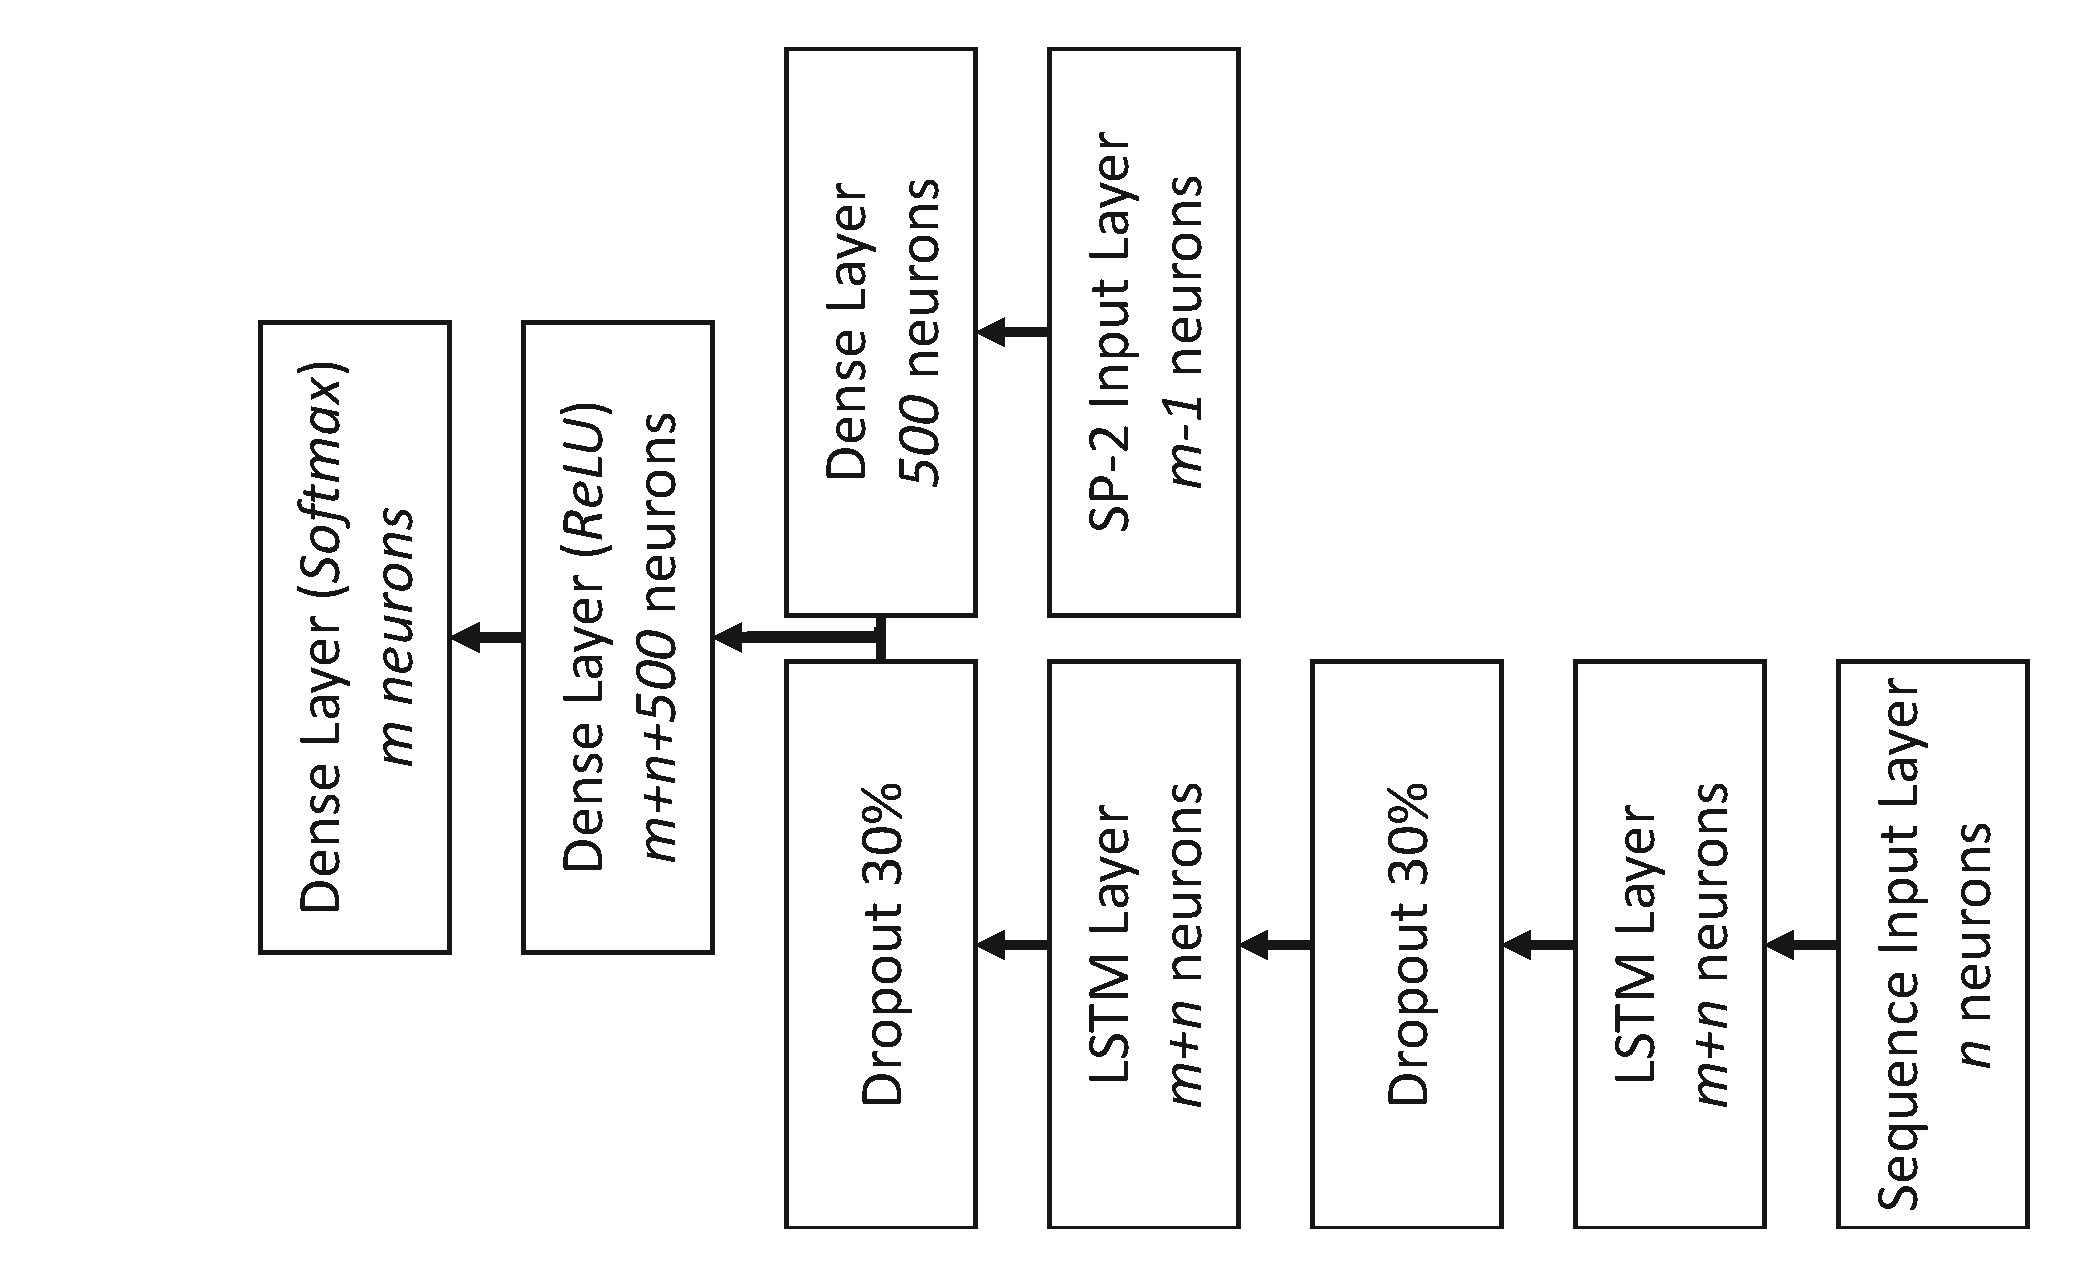
\includegraphics[width=.8\textwidth, angle=-90,origin=c]{gfx/sp2-network-architecture.pdf}
    \caption{The SP2 network architecture}
    \label{fig:sp2-architecture}
\end{figure}

\autoref{fig:sp2-architecture} displays the adapted network architecture from Shibata et al. It will be referred to as SP2 from here on.

We copied the bipartite structure and made small changes to dimensions and layers.
The sequential feature vectors, i.e. all event attributes, are fed in on the left input layer.
$n$ indicates the dimensionality of a feature vector.
The sequential data passes through two LSTM layers interleaved with dropout layers to prevent overfitting.
Hidden layers adapt their size $n+m$ to the input and output dimensions dimensions.
The LSTM layer output is concatenated with the output of the processed SP-2 features for each timestep.
The SP-2 features are fed in on the right side of the tree.
The concatenated vectors are passed through a ReLU activation function, and
finally to the output layer. The output layer uses a Softmax activation function,
and puts out the next activity in one-hot encoded form through $m$ units.
This models the problem as a multi-classification problem.

The Softmax activation function is commonly used to produce classification output,
while the ReLU activation function benefits training speeds~\cite{krizhevsky2012imagenet}.

In contrast to the original model, we completely removed the Embedding layers.
Above the SP-2 feature input layer, the Embedding layer was replaced with a fully-connected layer.
The reason for the removal is as follows: Shibata et al. predicted the next word in a sentence based on the preceding words.
As each word is an item, the itemsets in the case of Shibata only consist of a single item~\cite{shibata2016bipartite}.
We aim to predict the next activity based on the preceding events.
As shown in the previous section, the event-itemsets consist of multiple items which represent different attributes.
Embedding layers require dictionary-encoded input of a single item, which is a problem when multiple items belong together~\cite{goldberg2014word2vec}. A second reason against using Embedding layers in this context is the dimensionality of the inputs. The count of activities in a process is small compared to the number of words that are processed with Embedding layers in NLP scenarios~\cite{goldberg2014word2vec}.

Another difference are the dimensions of the hidden layers: In contrast to Evermann et al. and Shibata et al., the size is not fixed or smaller than the output unit count $m$.
This follows general advice not to introduce bottlenecks in the hidden layers by using fewer units than required in the output layer~\cite{web:techniques-in-convnets,szegedy2016rethinking}.\\

\noindent The SP-2 features are to be engineered based on the activity names, as the name of the next activity is also the prediction target.
Shibata et al. also engineered SP-2 features based on the history of the prediction targets~\cite{shibata2016bipartite}.

\section{Encoding subsequence occurrence}\label{sec:contrib:pfs-inspiration}
Klinkmüller et al. compared different feature representations and found that features that encode sub-trace occurrence can help models cover a broader variety of relationships~\cite{klinkmuller2018reliablemonitoring}.
While they found this to be true for random forests, we want to investigate the applicability of such features for LSTM neural networks.
Francescomarino et al. tried this in their work, and achieved discouraging accuracies around $0.50$~\cite{francescomarino2017}.
We are convinced that another network architecture could make a difference.

SP-2 features already encode history and subsequence encodings do the same on a higher level of abstraction.
Therefore, we take the SP2 model architecture and inject different features in place of the SP-2 features.
Said features and the corresponding architecture will henceforth be referred to as PFS, as illustrated in \autoref{fig:pfs-architecture}. The PFS feature vector has $l$ dimensions.
The acronym PFS originates from the word PrefixSpan, which is the name of the algorithm that we use in \autoref{chap:evaluation} to mine the subsequences.

\begin{figure}[ht]
    \centering
    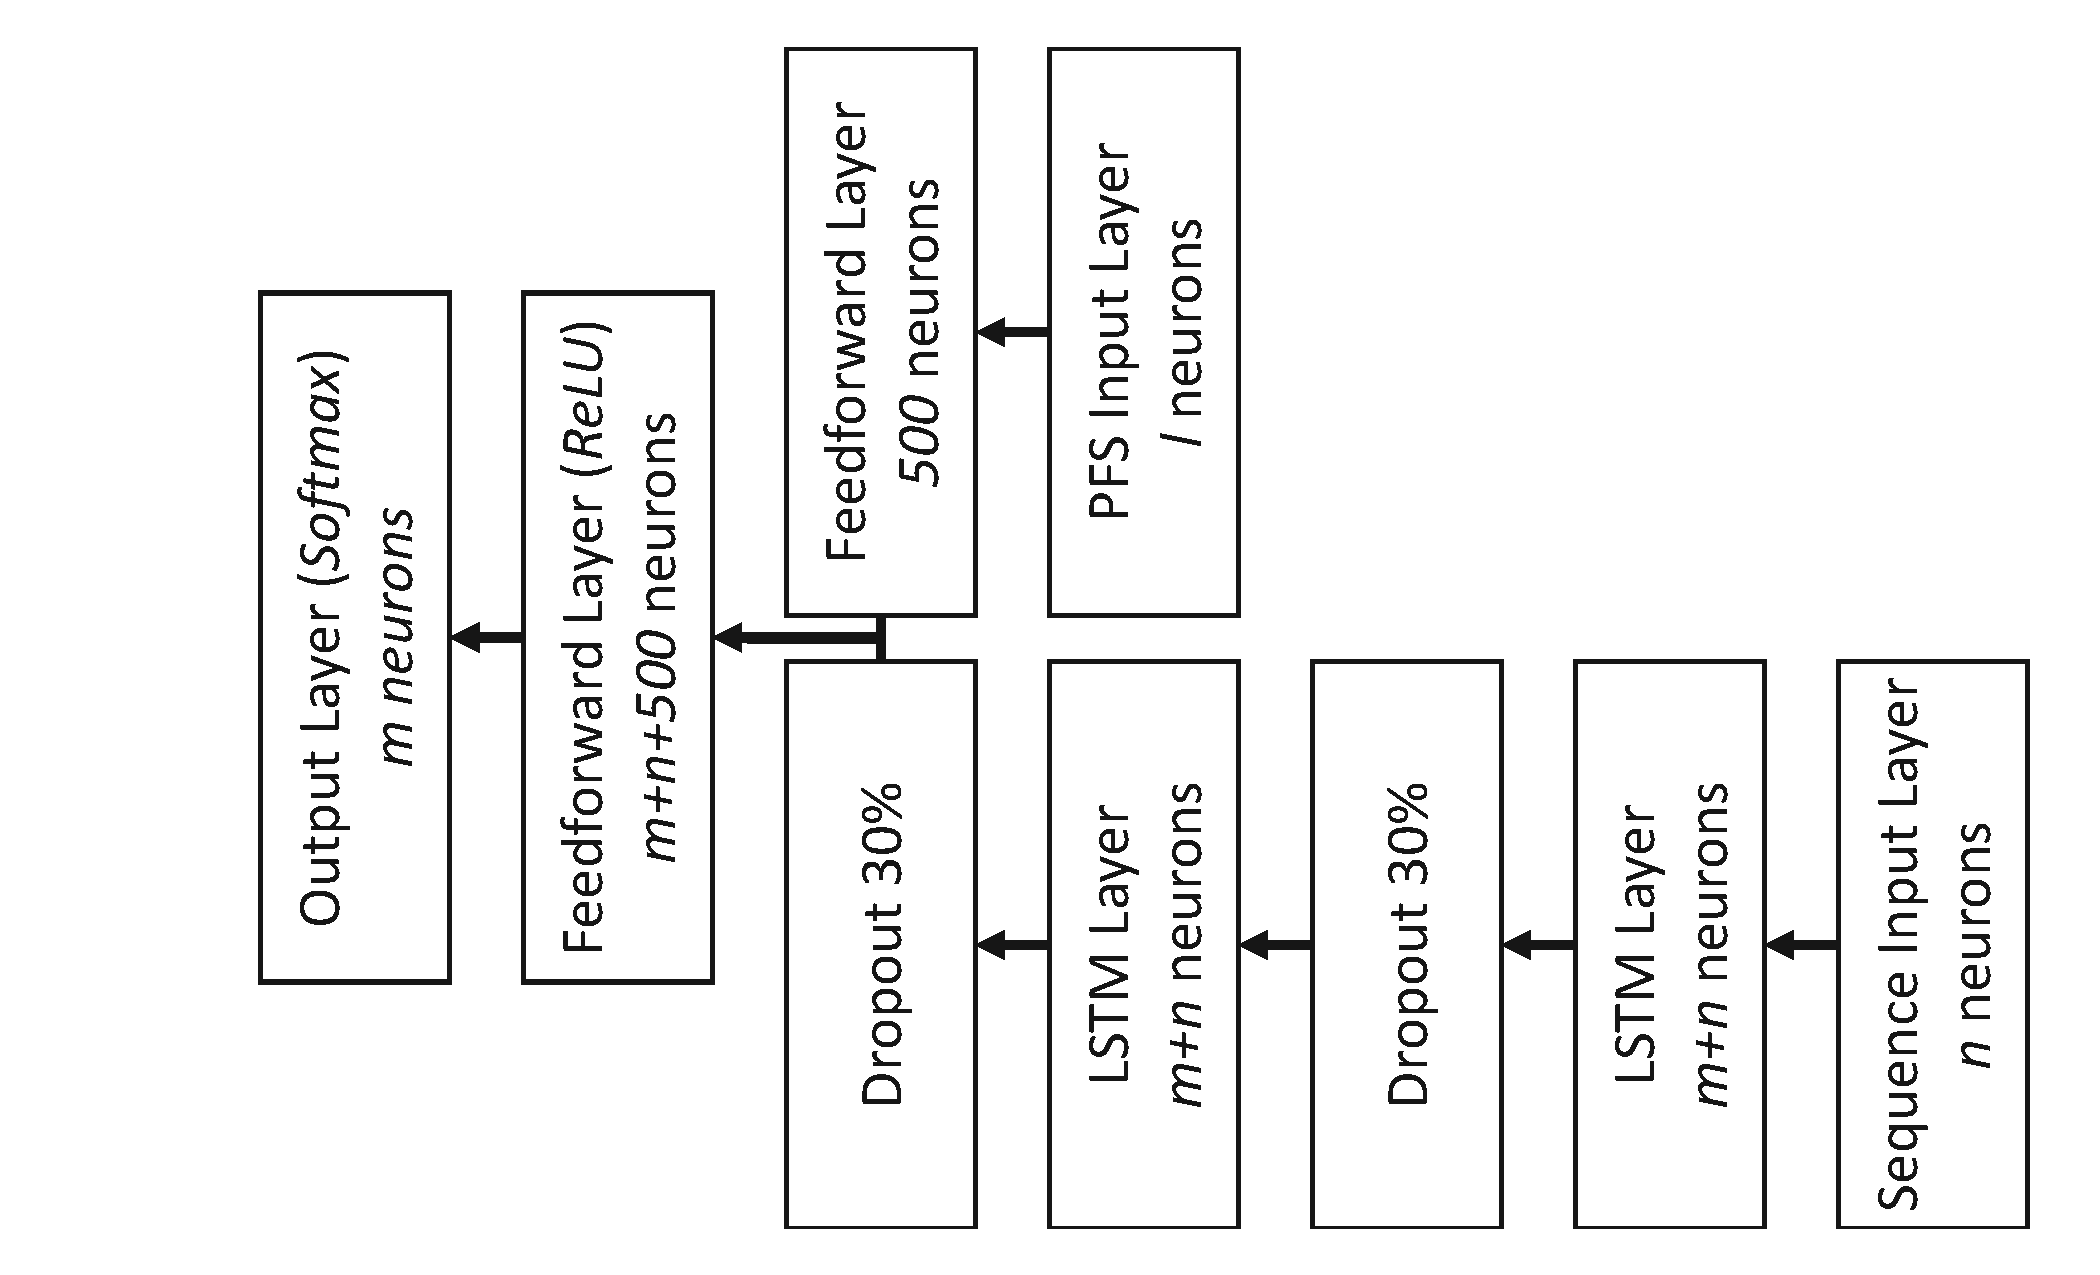
\includegraphics[width=.8\textwidth,angle=-90,origin=c]{gfx/pfs-network-architecture.pdf}
    \caption{The PFS network architecture}
    \label{fig:pfs-architecture}
\end{figure}

We presented two neural network architectures in this chapter. They incorporate
learnings from a successful NLP competition submission, and a paper on feature engineering.
Training these models on a multitude of datasets presented us with a challenge.
We solved it by constructing a small training framework which we present in the next chapter.
